\documentclass[12pt]{article}
\usepackage{amsmath, amssymb}
\usepackage{physics}
\usepackage{xcolor}
\usepackage{tikz}
\usepackage{pgfplots}
\pgfplotsset{compat=1.17}
\usepackage[margin=1in]{geometry}

\title{Gaussian Pulse Propagation in Optical Fibers: \\
A Complete, Intuitive Explanation}
\author{Step-by-Step Derivation with Physical Insight}
\date{\today}

\begin{document}

\maketitle

\tableofcontents

\section{The Big Picture: What Happens to a Pulse?}

\subsection{The Question}

When you send a short laser pulse (like 10 picoseconds) through an optical fiber, what happens to it?
\textbf{Answer:} Three main effects:
\begin{enumerate}
\item \textbf{Delay}: The pulse takes time to propagate (travels at group velocity)
\item \textbf{Broadening}: The pulse spreads out in time (due to dispersion)
\item \textbf{Attenuation}: The pulse weakens (due to loss)
\end{enumerate}

\subsection{Why Gaussian Pulses?}

Gaussian pulses are important because:
\begin{itemize}
\item Many lasers naturally produce Gaussian-shaped pulses
\item Mathematically tractable (Gaussian $\leftrightarrow$ Gaussian under Fourier transform)
\item Good model for real pulse shapes
\item Preserves shape during linear propagation (only width changes)
\end{itemize}

\section{Starting Point: The Input Pulse}

\subsection{Mathematical Form}

At the fiber input ($z = 0$), we have a Gaussian pulse:
\begin{equation}
\boxed{A(t, 0) = A_0 \exp\left(-\frac{t^2}{2T_0^2}\right) e^{i\omega_0 t}}
\end{equation}

Let's understand each part:

\begin{itemize}
\item $A_0$ = peak amplitude (V/m or similar)
\item $\exp(-t^2/2T_0^2)$ = Gaussian envelope (bell curve)
\item $T_0$ = \textbf{initial pulse width} (1/e half-width in amplitude)
\item $e^{i\omega_0 t}$ = fast oscillation at carrier frequency $\omega_0$
\end{itemize}

\subsection{Physical Picture}

\begin{center}
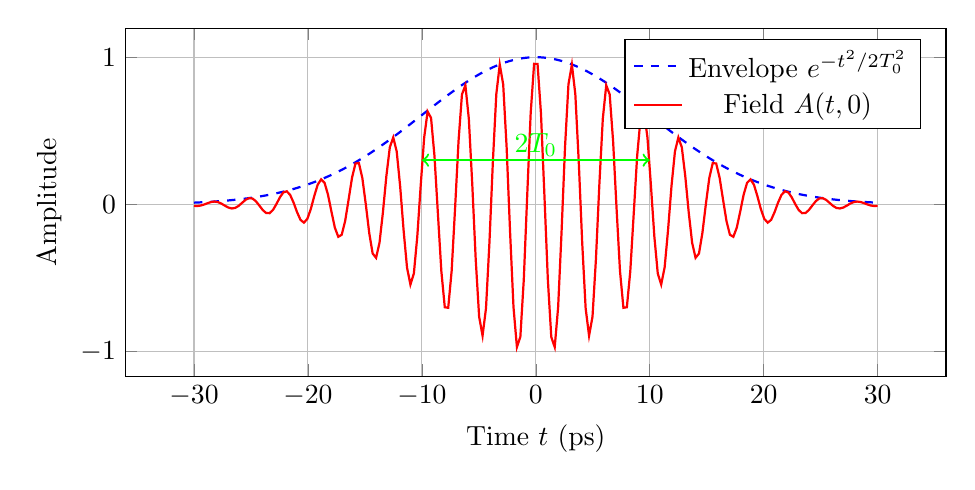
\begin{tikzpicture}
\begin{axis}[
    width=12cm, height=6cm,
    xlabel={Time $t$ (ps)},
    ylabel={Amplitude},
    domain=-30:30,
    samples=200,
    grid=major,
    legend pos=north east
]
% Gaussian envelope
\addplot[blue, thick, dashed] {exp(-x^2/200)};
\addlegendentry{Envelope $e^{-t^2/2T_0^2}$}

% Oscillating field
\addplot[red, thick] {exp(-x^2/200)*cos(deg(x*2))};
\addlegendentry{Field $A(t,0)$}

% Width marker
\draw[<->, green, thick] (axis cs:-10,0.3) -- (axis cs:10,0.3);
\node[green] at (axis cs:0,0.4) {$2T_0$};
\end{axis}
\end{tikzpicture}
\end{center}

\subsection{Pulse Width Definition}

The \textbf{full width at half maximum (FWHM)} is:
\begin{equation}
\text{FWHM} = 2\sqrt{2\ln 2} \, T_0 \approx 1.665 \, T_0
\end{equation}

So if $T_0 = 10$ ps, FWHM $\approx 16.65$ ps.

\section{The Key Tool: Fourier Transform}

\subsection{Why Use Fourier Transform?}

The propagation equation is simple in the \textbf{frequency domain}:
$$\tilde{A}(\omega, z) = \tilde{A}(\omega, 0) \cdot e^{i\beta(\omega)z}$$

Each frequency component just picks up a phase $e^{i\beta(\omega)z}$!
In the time domain, this would be a complicated convolution. Fourier transforms make it simple.

\subsection{Fourier Transform of Gaussian}

Starting with:
$$A(t, 0) = A_0 e^{-t^2/2T_0^2} e^{i\omega_0 t}$$

The Fourier transform is:
\begin{equation}
\tilde{A}(\omega, 0) = \frac{1}{\sqrt{2\pi}} \int_{-\infty}^\infty A(t,0) e^{i\omega t} dt
\end{equation}

\textbf{Key fact:} Fourier transform of Gaussian is Gaussian!
\begin{equation}
\boxed{\tilde{A}(\omega, 0) = A_0 T_0 \sqrt{2\pi} \exp\left(-\frac{(\omega - \omega_0)^2 T_0^2}{2}\right)}
\end{equation}

\subsection{Physical Interpretation}

\begin{center}
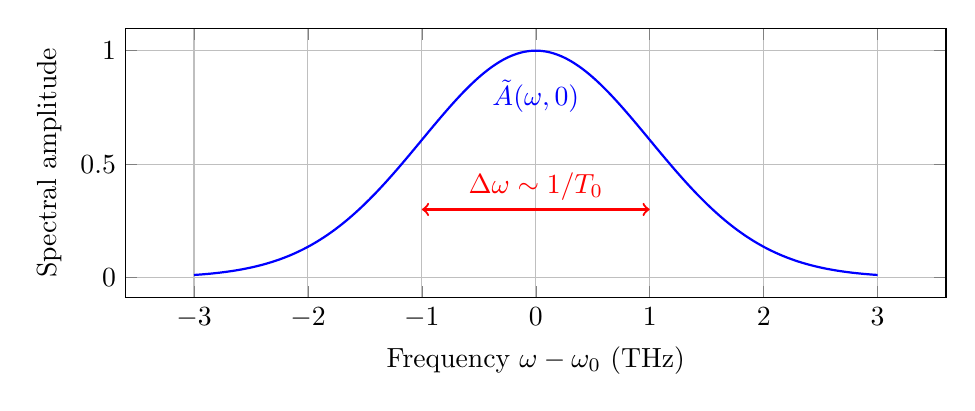
\begin{tikzpicture}
\begin{axis}[
    width=12cm, height=5cm,
    xlabel={Frequency $\omega - \omega_0$ (THz)},
    ylabel={Spectral amplitude},
    domain=-3:3,
    samples=200,
    grid=major
]
\addplot[blue, thick] {exp(-x^2/2)};
\node[blue] at (axis cs:0,0.8) {$\tilde{A}(\omega, 0)$};

% Bandwidth marker
\draw[<->, red, thick] (axis cs:-1,0.3) -- (axis cs:1,0.3);
\node[red] at (axis cs:0,0.4) {$\Delta\omega \sim 1/T_0$};
\end{axis}
\end{tikzpicture}
\end{center}

\textbf{Time-bandwidth product:}
$$\Delta t \cdot \Delta \omega \sim 1$$

Shorter pulse (small $T_0$) $\Rightarrow$ broader spectrum (large $\Delta\omega$)!

\section{Dispersion: The Taylor Series}

\subsection{What is Dispersion?}

Different frequencies travel at different speeds!
The propagation constant $\beta(\omega)$ tells us how fast each frequency propagates:
\begin{equation}
\beta(\omega) = \text{phase accumulated per unit length at frequency } \omega
\end{equation}

\subsection{Taylor Expansion}

Expand $\beta(\omega)$ around the carrier frequency $\omega_0$:
\begin{equation}
\boxed{\beta(\omega) = \beta_0 + \beta_1(\omega - \omega_0) + \frac{\beta_2}{2}(\omega - \omega_0)^2 + \frac{\beta_3}{6}(\omega - \omega_0)^3 + \cdots}
\end{equation}

\subsection{Physical Meaning of Each Term}

\begin{align}
\beta_0 &= \beta(\omega_0) \quad \text{\textcolor{blue}{Overall phase (unimportant for pulse shape)}} \\[0.3cm]
\beta_1 &= \frac{d\beta}{d\omega}\bigg|_{\omega_0} = \frac{1}{v_g} \quad \text{\textcolor{blue}{Inverse group velocity (delay)}} \\[0.3cm]
\beta_2 &= \frac{d^2\beta}{d\omega^2}\bigg|_{\omega_0} \quad \text{\textcolor{red}{Group velocity dispersion (GVD) (broadening!)}} \\[0.3cm]
\beta_3 &= \frac{d^3\beta}{d\omega^3}\bigg|_{\omega_0} \quad \text{\textcolor{blue}{Third-order dispersion (pulse asymmetry)}}
\end{align}

\subsection{Why $\beta_2$ Causes Broadening}

The $\beta_2$ term means:
$$\text{phase} \sim \frac{\beta_2}{2}(\omega - \omega_0)^2 z$$

Different frequencies acquire \textbf{different phases}!
\begin{itemize}
\item Red frequencies ($\omega < \omega_0$): one phase
\item Blue frequencies ($\omega > \omega_0$): different phase
\end{itemize}

When we inverse Fourier transform, these phase differences cause the pulse to spread out.

\section{Propagation in Frequency Domain}

\subsection{Propagation Formula}

After propagating distance $z$:
\begin{equation}
\tilde{A}(\omega, z) = \tilde{A}(\omega, 0) \cdot e^{i\beta(\omega)z} \cdot e^{-\alpha z/2}
\end{equation}

Keeping only up to $\beta_2$:
\begin{equation}
\tilde{A}(\omega, z) = \tilde{A}(\omega, 0) \cdot \exp\left[i\beta_0 z + i\beta_1(\omega-\omega_0)z + \frac{i\beta_2}{2}(\omega-\omega_0)^2 z\right]
\end{equation}

\subsection{Substituting the Gaussian}

\begin{align}
\tilde{A}(\omega, z) &= A_0 T_0 \sqrt{2\pi} \exp\left[-\frac{(\omega-\omega_0)^2 T_0^2}{2}\right] \notag \\
&\quad \times \exp\left[i\beta_0 z + i\beta_1(\omega-\omega_0)z + \frac{i\beta_2}{2}(\omega-\omega_0)^2 z\right]
\end{align}

Combining the exponentials:
\begin{equation}
\tilde{A}(\omega, z) = A_0 T_0 \sqrt{2\pi} e^{i\beta_0 z} \exp\left[-\frac{(\omega-\omega_0)^2 T_0^2}{2} + i\beta_1(\omega-\omega_0)z + \frac{i\beta_2 z}{2}(\omega-\omega_0)^2\right]
\end{equation}

% ---------------------------------------------------------
% CORRECTED SECTIONS START HERE
% ---------------------------------------------------------

\section{The Magic: Completing the Square}

\subsection{Combining Terms}

Define $\Omega = \omega - \omega_0$ for simplicity.
The exponent in the equation above is:
\begin{equation}
-\frac{\Omega^2 T_0^2}{2} + i\beta_1 \Omega z + \frac{i\beta_2 z}{2}\Omega^2
\end{equation}

Factor out the $\Omega^2$ terms:
\begin{equation}
= -\frac{1}{2}\left(T_0^2 - i\beta_2 z\right)\Omega^2 + i\beta_1 z \Omega
\end{equation}

Define the complex pulse width parameter:
\begin{equation}
T^2(z) = T_0^2 - i\beta_2 z
\end{equation}

Substituting this back, we get a concise quadratic form (note that $T^2(z)$ is in the numerator):
\begin{equation}
\boxed{\text{Exponent} = -\frac{1}{2}T^2(z)\Omega^2 + i\beta_1 z \Omega}
\end{equation}

\subsection{Completing the Square}

We want to write this quadratic in the standard form $-a(\Omega - k)^2 + C$ to prepare it for integration.

\textbf{Standard form:} $-a\Omega^2 + b\Omega = -a\left(\Omega - \frac{b}{2a}\right)^2 + \frac{b^2}{4a}$

Identifying our coefficients:
\begin{itemize}
    \item $a = \frac{T^2(z)}{2}$
    \item $b = i\beta_1 z$
\end{itemize}

Applying the standard form:
\begin{equation}
\text{Square Term} = -\frac{T^2(z)}{2}\left(\Omega - \frac{i\beta_1 z}{T^2(z)}\right)^2
\end{equation}

And the constant term (which comes out of the square):
\begin{equation}
\text{Constant} = \frac{b^2}{4a} = \frac{(i\beta_1 z)^2}{4(T^2(z)/2)} = \frac{-\beta_1^2 z^2}{2T^2(z)}
\end{equation}

Thus, the full exponent is:
\begin{equation}
-\frac{T^2(z)}{2}\left(\Omega - \frac{i\beta_1 z}{T^2(z)}\right)^2 - \frac{\beta_1^2 z^2}{2T^2(z)}
\end{equation}

\section{Inverse Fourier Transform: The Gaussian Integral}

\subsection{The Integral}

We now perform the inverse Fourier transform to get back to the time domain:
\begin{equation}
A(t, z) = \frac{1}{\sqrt{2\pi}} \int_{-\infty}^\infty \tilde{A}(\omega, z) e^{-i\omega t} d\omega
\end{equation}

Substituting $\omega = \Omega + \omega_0$ and our completed square form:
\begin{equation}
A(t, z) = \frac{A_0 T_0 \sqrt{2\pi}}{\sqrt{2\pi}} e^{i(\beta_0 z - \omega_0 t)} e^{-\frac{\beta_1^2 z^2}{2T^2(z)}} \int_{-\infty}^\infty \exp\left[-\frac{T^2(z)}{2}\left(\Omega - \frac{i\beta_1 z}{T^2(z)}\right)^2\right] e^{-i\Omega t} d\Omega
\end{equation}

\subsection{Solving the Integral}

This integral is the Fourier transform of a shifted Gaussian. We can solve it by shifting the integration variable $u = \Omega - \frac{i\beta_1 z}{T^2(z)}$.

The standard Gaussian integral result is:
\begin{equation}
\int_{-\infty}^\infty e^{-Au^2} e^{-iut} du = \sqrt{\frac{\pi}{A}} e^{-t^2/4A}
\end{equation}

Here, $A = T^2(z)/2$. The result of the integration is:
\begin{equation}
\text{Integral} = \sqrt{\frac{2\pi}{T^2(z)}} \exp\left[-\frac{(t - \beta_1 z)^2}{2T^2(z)}\right]
\end{equation}
\textit{(Note: The $(t-\beta_1 z)$ term arises from combining the external constant term and the Fourier phase shift.)}

\subsection{The Final Amplitude Expression}

Combining all prefactors and exponents:
\begin{equation}
\boxed{A(t, z) = \frac{A_0 T_0}{\sqrt{T^2(z)}} \exp\left[-\frac{(t - \beta_1 z)^2}{2T^2(z)}\right] e^{i(\beta_0 z - \omega_0 t)}}
\end{equation}

Substituting $T^2(z) = T_0^2(1 - i\beta_2 z/T_0^2)$:
\begin{equation}
A(t, z) = \frac{A_0}{\sqrt{1 - i\beta_2 z/T_0^2}} \exp\left[-\frac{(t - \beta_1 z)^2}{2T_0^2(1 - i\beta_2 z/T_0^2)}\right] e^{i(\beta_0 z - \omega_0 t)}
\end{equation}

\section{Pulse Width Evolution: The Key Result}

\subsection{Separating Real and Imaginary Parts}

The exponent governing the pulse shape is:
\begin{equation}
-\frac{(t - \beta_1 z)^2}{2T^2(z)}
\end{equation}

To find the physical pulse width, we must extract the real part of $1/T^2(z)$:
\begin{equation}
\frac{1}{T^2(z)} = \frac{1}{T_0^2 - i\beta_2 z} = \frac{T_0^2 + i\beta_2 z}{(T_0^2 - i\beta_2 z)(T_0^2 + i\beta_2 z)} = \frac{T_0^2 + i\beta_2 z}{T_0^4 + \beta_2^2 z^2}
\end{equation}

The real part of the exponent is therefore:
\begin{equation}
\text{Re}\left[-\frac{(t - \beta_1 z)^2}{2T^2(z)}\right] = -\frac{(t - \beta_1 z)^2}{2} \cdot \frac{T_0^2}{T_0^4 + \beta_2^2 z^2}
\end{equation}

We rewrite this in the standard Gaussian form $- \frac{(t - \beta_1 z)^2}{2T(z)^2}$:
\begin{equation}
\frac{1}{T(z)^2} = \frac{T_0^2}{T_0^4 + \beta_2^2 z^2} \implies T(z)^2 = \frac{T_0^4 + \beta_2^2 z^2}{T_0^2}
\end{equation}

\subsection{Dispersion Length and Final Width}

Dividing through by $T_0^2$:
\begin{equation}
T(z)^2 = T_0^2 \left(1 + \frac{\beta_2^2 z^2}{T_0^4}\right)
\end{equation}

Defining the \textbf{Dispersion Length} $L_D = \frac{T_0^2}{|\beta_2|}$, we get the famous broadening formula:

\begin{equation}
\boxed{T(z) = T_0 \sqrt{1 + \left(\frac{z}{L_D}\right)^2}}
\end{equation}

% ---------------------------------------------------------
% ORIGINAL SECTIONS RESUME HERE
% ---------------------------------------------------------

\subsection{Physical Interpretation}

\begin{center}
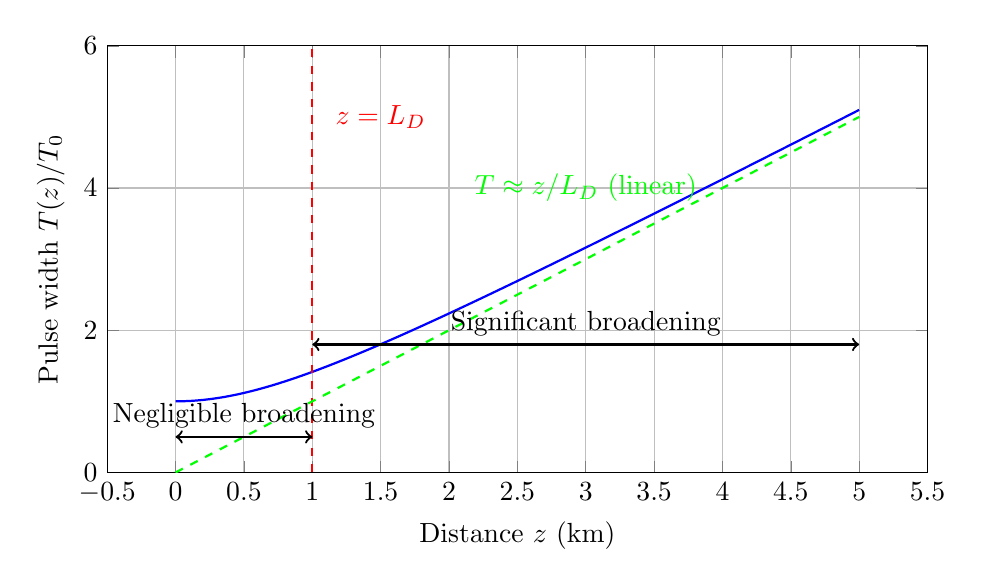
\begin{tikzpicture}
\begin{axis}[
    width=12cm, height=7cm,
    xlabel={Distance $z$ (km)},
    ylabel={Pulse width $T(z)/T_0$},
    domain=0:5,
    samples=100,
    grid=major,
    ymin=0, ymax=6
]
% Pulse width evolution
\addplot[blue, thick] {sqrt(1 + x^2)};
% Dispersion length marker
\draw[red, dashed, thick] (axis cs:1,0) -- (axis cs:1,6);
\node[red] at (axis cs:1.5,5) {$z = L_D$};
% Asymptote
\addplot[green, dashed, thick] {x};
\node[green] at (axis cs:3,4) {$T \approx z/L_D$ (linear)};
% Annotations
\draw[<->, thick] (axis cs:0,0.5) -- (axis cs:1,0.5);
\node at (axis cs:0.5,0.8) {Negligible broadening};
\draw[<->, thick] (axis cs:1,1.8) -- (axis cs:5,1.8);
\node at (axis cs:3,2.1) {Significant broadening};
\end{axis}
\end{tikzpicture}
\end{center}

\textbf{Three regimes:}

\begin{enumerate}
\item \textbf{$z \ll L_D$:} Negligible broadening
$$T(z) \approx T_0$$

\item \textbf{$z = L_D$:} $\sqrt{2}$ broadening (41\% increase)
$$T(L_D) = \sqrt{2} T_0$$

\item \textbf{$z \gg L_D$:} Linear broadening
$$T(z) \approx \frac{|\beta_2|z}{T_0}$$
\end{enumerate}

\section{Complete Picture: Delay + Broadening + Loss}

\subsection{Three Effects Combined}

\begin{equation}
\boxed{A(t, z) = \frac{A_0 e^{-\alpha z/2}}{\sqrt{1 - i\beta_2 z/T_0^2}} \exp\left[-\frac{(t - \beta_1 z)^2}{2T_0^2(1 - i\beta_2 z/T_0^2)}\right] e^{i(\beta_0 z - \omega_0 t)}}
\end{equation}

\begin{center}
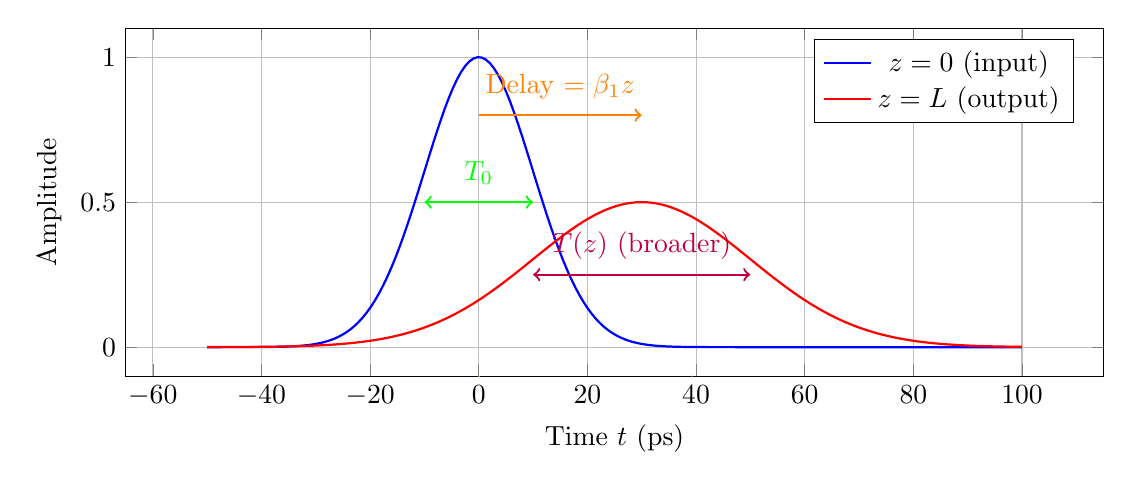
\begin{tikzpicture}
\begin{axis}[
    width=14cm, height=6cm,
    xlabel={Time $t$ (ps)},
    ylabel={Amplitude},
    domain=-50:100,
    samples=200,
    grid=major,
    legend pos=north east
]
% Input pulse at z=0
\addplot[blue, thick] {exp(-x^2/200)};
\addlegendentry{$z = 0$ (input)}

% After propagation
\addplot[red, thick] {0.5*exp(-(x-30)^2/800)};
\addlegendentry{$z = L$ (output)}

% Annotations
\draw[<->, green, thick] (axis cs:-10,0.5) -- (axis cs:10,0.5);
\node[green] at (axis cs:0,0.6) {$T_0$};

\draw[<->, purple, thick] (axis cs:10,0.25) -- (axis cs:50,0.25);
\node[purple] at (axis cs:30,0.35) {$T(z)$ (broader)};
\draw[->, orange, thick] (axis cs:0,0.8) -- (axis cs:30,0.8);
\node[orange] at (axis cs:15,0.9) {Delay $= \beta_1 z$};
\draw[->, brown, thick] (axis cs:0,-0.1) -- (axis cs:0,-0.2);
\node[brown] at (axis cs:20,-0.15) {Amplitude $\times e^{-\alpha z/2}$};
\end{axis}
\end{tikzpicture}
\end{center}

\subsection{Summary of Effects}

\begin{center}
\begin{tabular}{|l|l|l|}
\hline
\textbf{Effect} & \textbf{Parameter} & \textbf{Result} \\
\hline
Delay & $\beta_1 = 1/v_g$ & Peak shifts to $t = \beta_1 z$ \\
\hline
Broadening & $\beta_2$ (GVD) & Width increases: $T(z) = T_0\sqrt{1 + (z/L_D)^2}$ \\
\hline
Attenuation & $\alpha$ & Amplitude decreases: $A \to A e^{-\alpha z/2}$ \\
\hline
\end{tabular}
\end{center}

\section{Worked Example: Real Numbers}

\subsection{Problem Setup}

A fiber with:
\begin{itemize}
\item Length: $L = 10$ km
\item Core index: $n_{\text{core}} = 1.45$
\item GVD: $\beta_2 = -20$ ps$^2$/km
\item Attenuation: $\alpha = 0.2$ dB/km
\item Input pulse width: $T_0 = 10$ ps
\item Wavelength: $\lambda_0 = 1550$ nm
\end{itemize}

\subsection{Solution Step-by-Step}

\textbf{(a) Propagation delay:}
\begin{align}
\Delta t &= \beta_1 L = \frac{n_{\text{core}} L}{c} \\
&= \frac{1.45 \times 10^4 \text{ m}}{3 \times 10^8 \text{ m/s}} \\
&= 4.833 \times 10^{-5} \text{ s} = \boxed{48.33 \text{ }\mu\text{s}}
\end{align}

\textbf{(b) Dispersion length:}
\begin{align}
L_D &= \frac{T_0^2}{|\beta_2|} = \frac{(10 \text{ ps})^2}{20 \text{ ps}^2/\text{km}} \\
&= \boxed{5 \text{ km}}
\end{align}

\textbf{(c) Output pulse width:}
\begin{align}
T(L) &= T_0 \sqrt{1 + \left(\frac{L}{L_D}\right)^2} \\
&= 10 \sqrt{1 + \left(\frac{10}{5}\right)^2} \\
&= 10\sqrt{1 + 4} = 10\sqrt{5} \\
&= \boxed{22.36 \text{ ps}}
\end{align}

Broadening factor: $T(L)/T_0 = 2.236$ (124\% increase!)

\textbf{(d) Amplitude attenuation:}
\begin{align}
\alpha_{\text{Np}} &= 0.1151 \times 0.2 = 0.02302 \text{ Np/km} \\
A(L) &= A_0 e^{-\alpha_{\text{Np}} L} = A_0 e^{-0.2302} \\
&= \boxed{0.794 \, A_0}
\end{align}

Power: $P(L) = P_0 \times (0.794)^2 = 0.631 P_0$ (63.1\% remains)

\subsection{Visualization}

\begin{center}
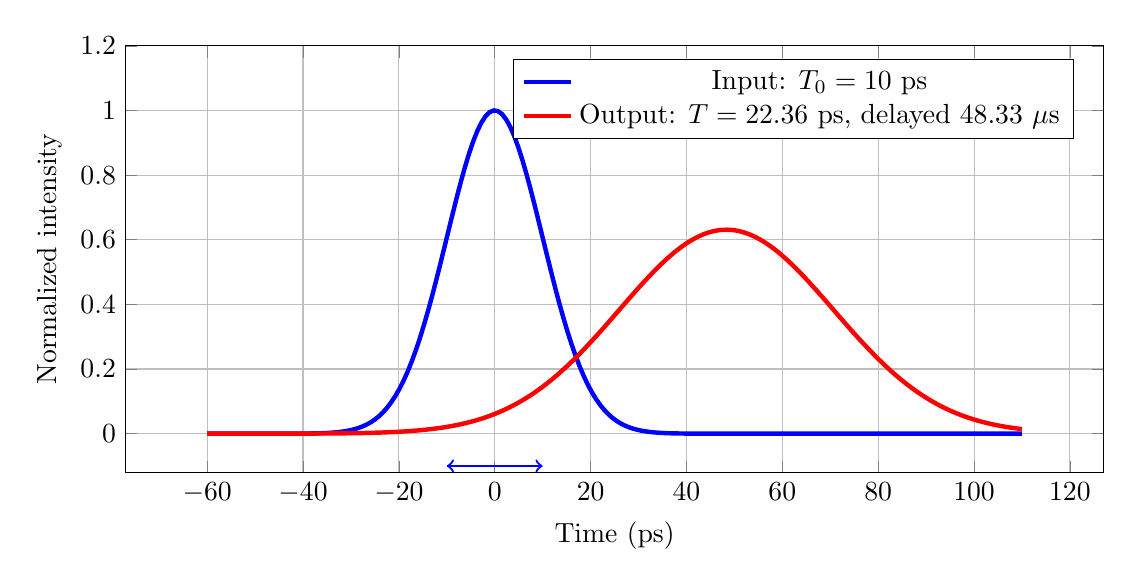
\begin{tikzpicture}
\begin{axis}[
    width=14cm, height=7cm,
    xlabel={Time (ps)},
    ylabel={Normalized intensity},
    domain=-60:110,
    samples=200,
    grid=major,
    legend pos=north east,
    ymax=1.2
]
% Input pulse
\addplot[blue, ultra thick] {exp(-x^2/200)};
\addlegendentry{Input: $T_0 = 10$ ps}

% Output pulse (delayed, broadened, attenuated)
\addplot[red, ultra thick] {0.631*exp(-(x-48330/1000)^2/1000)};
\addlegendentry{Output: $T = 22.36$ ps, delayed 48.33 $\mu$s}

% Width markers
\draw[<->, blue, thick] (axis cs:-10,-0.1) -- (axis cs:10,-0.1);
\node[blue] at (axis cs:0,-0.2) {FWHM $\approx$ 16.7 ps};

\end{axis}
\end{tikzpicture}
\end{center}

\section{Physical Insights}

\subsection{Why Does the Pulse Broaden?}

Think of the pulse as containing many frequency components:

\begin{enumerate}
\item \textbf{Red components} ($\omega < \omega_0$): travel slower (if $\beta_2 < 0$)
\item \textbf{Blue components} ($\omega > \omega_0$): travel faster (if $\beta_2 < 0$)
\end{enumerate}

Initially, all components are synchronized (constructive interference at $t=0$).
After propagation, they're out of sync → pulse spreads!

\subsection{Sign of $\beta_2$}

\begin{itemize}
\item \textbf{$\beta_2 < 0$ (normal dispersion):} Blue faster than red
\item \textbf{$\beta_2 > 0$ (anomalous dispersion):} Red faster than blue
\item \textbf{$\beta_2 = 0$:} Zero-dispersion wavelength (no broadening!)
\end{itemize}

For standard silica fiber:
\begin{itemize}
\item $\lambda < 1.3$ $\mu$m: $\beta_2 < 0$ (normal)
\item $\lambda = 1.3$ $\mu$m: $\beta_2 = 0$ (zero-dispersion)
\item $\lambda > 1.3$ $\mu$m: $\beta_2 > 0$ (anomalous)
\end{itemize}

\subsection{Chirp: Frequency Sweep}

The output pulse has a \textbf{chirp} - instantaneous frequency varies with time!
For $\beta_2 < 0$:
\begin{itemize}
\item Leading edge: lower frequency (red)
\item Trailing edge: higher frequency (blue)
\end{itemize}

This is why you can compress a chirped pulse with a grating!

\section{Engineering Applications}

\subsection{Dispersion Compensation}

To transmit over long distances without broadening:

\begin{enumerate}
\item \textbf{Dispersion-shifted fiber:} Design for $\beta_2 = 0$ at operating wavelength
\item \textbf{Dispersion compensation:} Use fiber with opposite $\beta_2$
\item \textbf{Pre-chirping:} Chirp pulse before transmission so dispersion compresses it
\end{enumerate}

\subsection{Bit Rate Limits}

For digital communication, pulses must not overlap.
If pulse width after distance $L$ is $T(L)$, bit rate is limited by:
\begin{equation}
B < \frac{1}{2T(L)} = \frac{1}{2T_0\sqrt{1 + (L/L_D)^2}}
\end{equation}

For $L \gg L_D$:
\begin{equation}
B < \frac{T_0}{2|\beta_2|L}
\end{equation}

\subsection{Dispersion-Bit Rate Product}

A key figure of merit:
\begin{equation}
B \cdot L < \frac{1}{2|\beta_2|B}
\end{equation}

Example: For $\beta_2 = -20$ ps$^2$/km and $B = 10$ Gb/s:
\begin{equation}
L < \frac{1}{2 \times 20 \times 10^{-24} \times 10^{10}} = 2500 \text{ km}
\end{equation}

\section{Connection to Quantum Communication}

In quantum communication, these same effects apply to quantum states:

\begin{equation}
|\alpha(0)\rangle \xrightarrow{\text{propagate}} |\alpha(L)\rangle
\end{equation}

where:
\begin{equation}
\alpha(L) = \alpha(0) e^{i\beta(\omega)L} e^{-\alpha L/2}
\end{equation}

The dispersion causes:
\begin{itemize}
\item Phase uncertainty
\item Timing jitter
\item Reduced distinguishability of quantum states
\end{itemize}

All affecting channel capacity!

\section{Summary: Key Equations}

\begin{align}
\text{Input:} \quad & A(t,0) = A_0 e^{-t^2/2T_0^2} e^{i\omega_0 t} \\[0.3cm]
\text{Dispersion length:} \quad & L_D = \frac{T_0^2}{|\beta_2|} \\[0.3cm]
\text{Output width:} \quad & T(z) = T_0\sqrt{1 + (z/L_D)^2} \\[0.3cm]
\text{Delay:} \quad & \Delta t = \beta_1 z = \frac{n_{\text{eff}} z}{c} \\[0.3cm]
\text{Attenuation:} \quad & A \to A e^{-\alpha z/2} \\[0.3cm]
\text{Complete output:} \quad & A(t,z) = \frac{A_0 e^{-\alpha z/2}}{\sqrt{1-i\beta_2 z/T_0^2}} \exp\left[-\frac{(t-\beta_1 z)^2}{2T_0^2(1-i\beta_2 z/T_0^2)}\right] e^{i(\beta_0 z - \omega_0 t)}
\end{align}

\end{document}